\chapter{Background and Related Work} \label{chap:relatedwork}

The background chapter of this paper focuses on the use of \acrshort{nerf}s for representing and rendering 3D scenes. The chapter discusses several important NeRF methods, including NeRF \cite{mildenhall_nerf_2020}, Mip-NeRF \cite{barron_mip-nerf_2021}, mip-NeRF 360 \cite{barron_mip-nerf_2022}, Block-NeRF \cite{tancik_block-nerf_2022}, and Instant-ngp \cite{muller_instant_2022}. Additionally, the chapter covers several key techniques used in the NeRF pipeline, including positional encoding, hierarchical sampling, stratified sampling, appearance embeddings, learned pose refinement, and visibility prediction.

The chapter also discusses the use of \acrfull{sfm} and COLMAP \cite{schonberger_structure--motion_2016} as important tools for the pre-processing step in the NeRF pipeline, and presents several metrics for evaluating NeRFs. By providing an overview of these methods, techniques, tools, and metrics, the background chapter aims to establish a common ground for future chapters.

This thesis assumes a foundational understanding of deep learning. A great resource for individuals looking to acquire such knowledge is the publication by Goodfellow et al. \cite{Goodfellow}.

Please note that, in order to cover the relevant background, some sections of the following chapter have been adapted from my unpublished project work on NeRFs for novel view synthesis and 3D reconstruction, which was completed as part of the course “TDT4501 Computer Science, Specialization Project”.

% --------------------- Volume rendering ---------------------
\section{Volume Rendering} \label{sec:volumerendering}
% OLD SECTION
%Volume rendering is a technique for visualizing 3D data sets, such as those obtained from medical imaging scans. It works by computing a 2D projection of a 3D volume, using algorithms to assign colors and opacities to each point in the volume based on its physical characteristics, such as density or temperature. Many visual effects are volumetric in nature, e.g. fluids, clouds, flames, smoke, fog, and dust. These effects are challenging to simulate with geometric primitives like points, lines, triangles, or polygon meshes, and may be better simulated with volume rendering. A volume renderer may also be used to display not just the model's surfaces but all of its fine external and internal details, allowing the user to see inside the volume to get a better understanding of its internal structure. Because of this, volume rendering is a powerful tool for visualizing complex 3D data and can be used in a wide range of applications, including medical imaging, scientific visualization, and computer graphics \cite{max_optical_1995}.

% REWRITTEN WITH AI AND FURTHER EDITING ✅
Volume rendering is a powerful technique for visualizing 3D data sets, which is frequently used in a variety of fields, including medical imaging, scientific visualization, and computer graphics. The method involves the projection of a 3D volume onto a 2D plane, leveraging algorithms where colors and opacities are assigned to each point based on its physical characteristics, such as density or temperature. The resulting 2D image provides a representation of the entire 3D volume, allowing the user to visualize both the external and internal structure of the object. One of the main advantages of volume rendering is that it can simulate complex volumetric effects that are challenging to model using traditional geometric primitives, such as points, lines, triangles, or polygon meshes. Examples of such volumetric effects that may be better simulated with volume rendering include fluids, clouds, flames, smoke, fog, and dust \cite{max_optical_1995}.


% COMMENTS FROM SPECIALIZATION-PROJECT
%Volume rendering is a technique for visualizing 3D data sets, such as those obtained from medical imaging scans. It works by computing a 2D projection of a 3D volume, using algorithms to assign colors and opacities to each point in the volume based on its physical characteristics, such as density or temperature. A volume renderer may be used to display not just the model's surfaces but also all of its fine external and internal details, allowing the user to see inside the volume to get a better understanding of its internal structure. Many visual effects are volumetric in nature, and it is challenging to simulate fluids, clouds, flames, smoke, fog, and dust using geometric primitives. Such effects may be produced more effectively with volumetric models. \cite{ikits_chapter_2007}. Volume rendering is a powerful tool for visualizing complex 3D data and can be used in a wide range of applications, including medical imaging, scientific visualization, and computer graphics\cite{max_optical_1995}.

%"Direct volume rendering refers to techniques which produce a projected image directly from the volume data, without intermediate constructs such as contour surface polygons" \cite{max_optical_1995}. It makes it possible to project 2D images from a series of discretely sampled 3D data. A volume renderer may be used to display not just the model's surfaces but also all of its fine details. Many visual effects are volumetric in nature. It is challenging to simulate fluids, clouds, flames, smoke, fog, and dust using geometric primitives. Such effects may be produced more effectively with volumetric models. These models presuppose that a high number of particles in the volume emit, absorb, and scatter light \cite{ikits_chapter_2007}.

%After having acquired a 3D data set, rays are cast from the center of the viewing direction (camera origin), through the image plane and into the volume. As the ray enters the volume, an intensity profile is generated. The scalar value per the depth of the volume will be proportional with the density of the volume being traversed.
%Volume rendering enables photorealistic novel view synthesis \cite{xie_neural_2022}.

% ALMOST NOTHING REWRITTEN ❌ It's already very good.
There are multiple ways of rendering a volume. Well-known techniques include ray casting or raymarching, resampling or shear-warp, texture slicing, and splatting. The basic algorithm, depicted in \autoref{fig:volume-rendering}, can be broken into four steps:

\begin{itemize}
    \item \textbf{Ray casting:} Cast rays from the image plane into the volume. The volume is often enclosed within a bounding primitive like a cuboid.
    \item \textbf{Sampling:} As the ray enters the volume, sample equally spaced points from the volume. This equidistant sampling builds an intensity profile for the ray; density per volume depth. In the general case where the volume isn't aligned with the ray's direction, the sampling point will be positioned in between voxels, and the values must be interpolated from its adjacent voxels.
    \item \textbf{Shading:} Utilizing the generated intensity profile and a transfer function, compute the $RGB\alpha$-color and an illumination-value gradient. The gradient vector points in the direction of the greatest increase, indicating where the most rapid increase in illumination is. The samples are colored with their $RGB\alpha$ value and shaded according to the gradient vector and the location of the scene's light source.
    \item \textbf{Compositing:} The final color of the pixel is retrieved by compositing all the shaded samples along the ray. 
\end{itemize}

\begin{figure}[h]
    \centering
    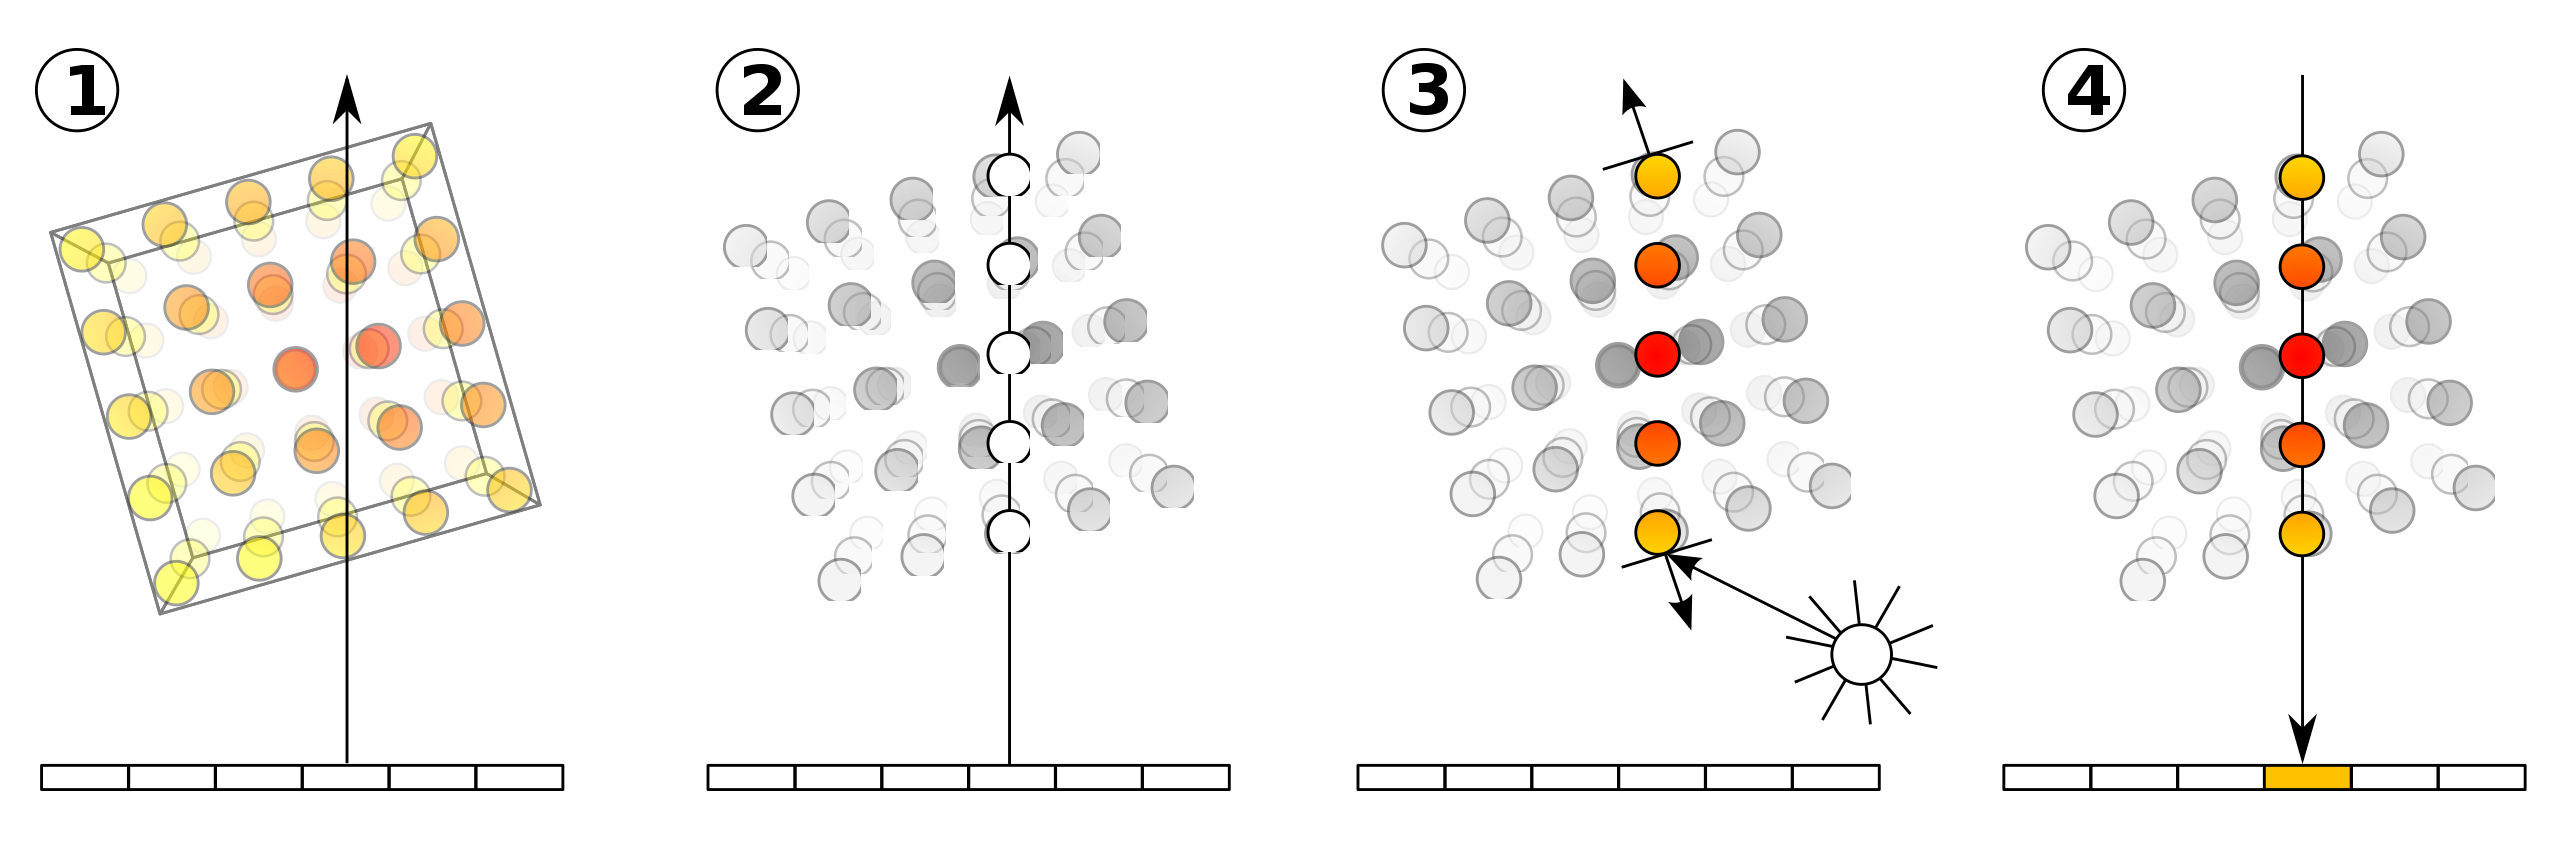
\includegraphics[width=1.0\textwidth]{figures/volume-rendering.png}
    \caption{The four basic steps of volume rendering \cite{wiki:Volume_ray_casting}. 1) A ray is cast from the image plane into the volume. 2) Points in the volume are sampled. 3) The points are shaded based on their $RGB\alpha$-value and the illumination-value gradients in relationship with the local light source. 4) The final pixel color is obtained by compositing all the shaded samples along the ray.}
    \label{fig:volume-rendering}
\end{figure}


\begin{comment}
\subsection{Alpha compositing}
Alpha compositing is the process of combining one image with a background to create the appearance of partial or full transparency \cite{wiki:Alpha_compositing}.

\subsection{Ray marching}
\end{comment}



% --------------------- Neural Fields ---------------------
\section{Neural Fields} % All text is taken from \cite{xie_neural_2022} - rewrite - have now paraphrased it
% ✅ SOMEWHAT REWRITTEN
A neural field refers to a field that has been parameterized, either entirely or partially, by a neural network. The field is a quantity that may be defined for any set of temporal or spatial coordinates. By design, neural fields are both continuous and adaptable. Neural fields are commonly parameterized as \acrlong{mlp}s (\acrshort{mlp}s) with gradient-defined activation functions \cite{xie_neural_2022}.

A typical neural fields algorithm in visual computing would first, across space-time, sample coordinates and feed them into a neural network to produce field quantities. The field quantities are samples from the desired reconstruction domain of the problem, which defines how we represent the world, such as a radiance field or another appropriate representation. Then, we apply a forward map to relate the reconstruction to the sensor domain, which defines how we observe the world, such as through an RGB image. In the sensor domain, supervision is available and we calculate the reconstruction error that guides the neural network optimization process by comparing the reconstructed signal to the sensor measurement. Important parts from the neural field algorithm are visualized in \autoref{fig:neural-field}.


% OLD
%A field that has been entirely or partially parameterized by a neural network is known as a neural field. The field is a quantity that may be defined for any set of temporal or spatial coordinates. By design, neural fields are both continuous and adaptable. Neural fields are commonly parameterized as MLPs with gradient-defined activation functions \cite{xie_neural_2022}.

%A typical neural fields algorithm in visual computing would first, across space-time, sample coordinates and feed them into a neural network to produce field quantities. The field quantities are samples from the desired reconstruction domain of our problem. Then, we apply a forward map to relate the reconstruction to the sensor domain (e.g. RGB image), where supervision is available. Finally, we calculate the reconstruction error or loss that guides the neural network optimization process by comparing the reconstructed signal to the sensor measurement. Important parts from the neural field algorithm are visualized in \autoref{fig:neural-field}.

\begin{figure}[!h]
    \centering
    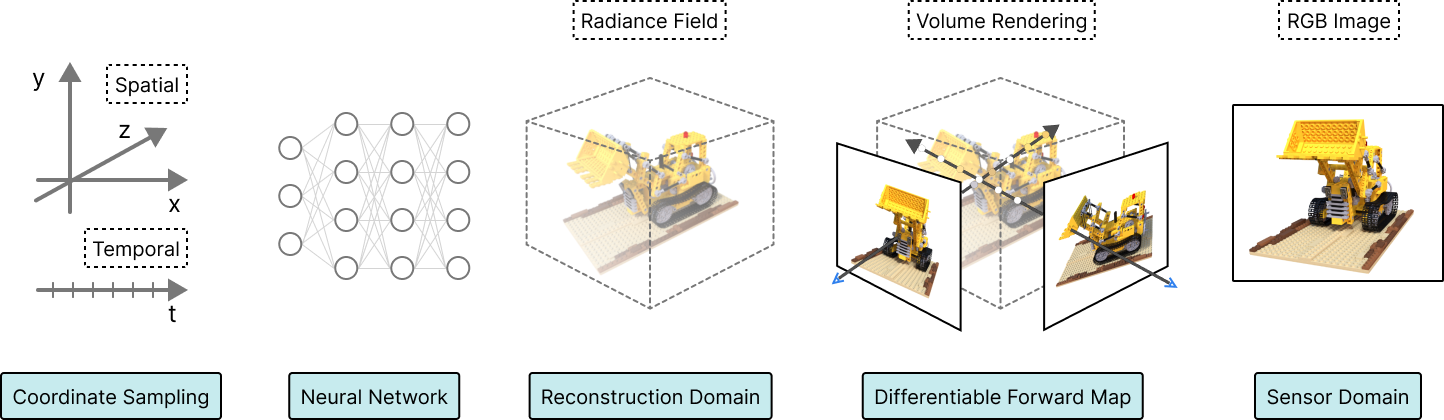
\includegraphics[width=1.0\textwidth]{figures/neural-field.png}
    \caption{Inspiration Figure 3 from Neural Fields in Visual Computing \cite{xie_neural_2022}. A typical neural fields algorithm in visual computing.}
    \label{fig:neural-field}
\end{figure}



% --------------------- Neural Radiance Fields (NeRFs) ---------------------
\subsection{Neural Radiance Fields}
% ✅ Somewhat rewritten, but mostly old.
The volumetric data we interact with through computer games, movies, and other computer graphic applications, are predominantly represented by meshes. A mesh is a collection of vertices, edges, and faces combined in order to define the shape of objects. Meshes are easy to manipulate and interact with. Another common representation of volume is voxels, where a 3D point in space is represented by a value, e.g. a color. Both of these modeling techniques are \textit{explicit} representations. As we want to increase the resolution of a scene, we have to model increasingly smaller regions of space, i.e. increase the number of voxels/triangle-meshes in the volume. This doesn't scale well as the memory requirements increase as we increase the number of voxels/triangle-meshes. Due to memory constraints, we have to find another way to represent the scene, instead of representing it as explicit blocks or meshes in space. NeRF provides an \textit{implicit} representation of the scene by utilizing an \acrshort{mlp}.

NeRF is a neural volumetric representation. The name, neural radiance fields, provides a clue as to what it is. It is a field, a space full of particles, where each particle has a given radiance, a color emitted by the particle in a certain direction, and the field is represented with a neural network. NeRF parameterizes 3D scenes as 3D neural fields, mapping 3D coordinates to radiance and density. The 3D scene can subsequently be rendered via volume rendering, as discussed in \autoref{sec:volumerendering}.

% OLD
%Most of the volumetric data we interact with through computer games, movies, and other computer graphic applications, are represented by meshes. A mesh is a collection of vertices, edges, and faces that can be combined in order to define the shape of objects. Meshes are easy to manipulate and interact with. Another common representation of volume is voxels, where a 3D point in space is represented by a value, e.g. a color. Both of these modeling techniques are explicit representations. As we want to increase the resolution of a scene, we have to model increasingly smaller regions of space, i.e. increase the number of voxels/triangle-meshes in the volume. This doesn't scale well as the memory requirements increase as we increase the number of voxels/triangle-meshes. We have to find another way to represent the scene, instead of representing it as explicit blocks in space. NeRF provides an implicit representation of the scene by utilizing a multi-layered perceptron (MLP).

%NeRF is a neural volumetric representation. The name, neural radiance fields, gives us a clue as to what it is. It is a field, a space full of particles, where each particle has a given radiance, a color emitted by the particle in a certain direction, and the field is represented with a neural network. NeRF parameterizes 3D scenes as 3D neural fields, mapping 3D coordinates to radiance and density. The 3D scene can subsequently be rendered via volume rendering, as discussed in \autoref{sec:volumerendering}.

\subsection{Differentiable Rendering} 
NeRFs are made possible due to differentiable rendering, a major breakthrough in 3D reconstruction. Differentiable rendering enables the rendering process to be implemented in a way that is amenable to gradient-based optimization. This in turn allows for the use of techniques such as backpropagation to optimize the parameters of a scene in order to produce a desired visual result. It allows reconstruction of 3D neural fields representing shape and/or appearance given only 2D images, instead of 3D supervision. This is particularly valuable as 3D data is often expensive to obtain, while 2D images are ubiquitous. As a result, non-experts can become 3D content creators without the barrier of specialized hardware, which has important social implications \cite{xie_neural_2022}.

% Differentiable rendering enables 3D content creation from omni-present 2D images, making it accessible to non-experts without specialized hardware. This has important social implications, as 3D data acquisition is often expensive. \cite{xie_neural_2022}.

%A major breakthrough in 3D reconstruction was the adoption of differentiable rendering (Section 4), which allowed reconstruction of 3D neural fields representing shape and/or appearance given only 2D images, instead of 3D supervision. This has significant implications since 3D data is often expensive to obtain, while 2D images are omni-present. A particularly important social implication is that non-experts can become 3D content creators, without the barrier of specialized hardware. \cite{xie_neural_2022}



% --------------------- NeRF ---------------------
% ✅ Somewhat rewritten
\section[NeRF]{NeRF - Representing Scenes as Neural Radiance Fields for View Synthesis} \label{sec:nerf}
The first paper to present NeRFs was \textit{NeRF - Representing Scenes as Neural Radiance Fields for View Synthesis} \cite{mildenhall_nerf_2020}. NeRFs provide a method for reconstructing 3D scenes and synthesizing novel views. Given multiple 2D images and their corresponding camera poses, NeRF builds a dataset by sampling points in the volume. The points in the dataset are passed through an \acrshort{mlp} in order to predict the given points' density and color. The predicted density and color values are then composited into a final color which is compared to the reference image pixel's color. The \acrshort{mlp} is optimized to minimize the difference between the predicted and reference pixel color.

%NeRF does this by querying an underlying MLP overfit to a specific scene, which represents a continuous volumetric field.
%NeRF renders pixels by emitting rays into the scene. The rays are represented by the ray equation $\pmb{r}(t) = \pmb{o} + t\pmb{d}$ where $\pmb{o}$ is the ray's origin, usually the center of the camera, and $\pmb{d}$ is the ray's direction.

Given multiple 2D images and their corresponding camera poses, which can be retrieved from calibrated camera rigs or approximated with \acrfull{sfm} techniques as will be discussed in \autoref{sec:colmap}, NeRF builds a dataset by sampling points in the volume. Points are sampled along a ray $\pmb{r}(t)$ with origin $\textbf{o}$, the camera's center of projection, and viewing direction $\textbf{d}$. The sampling rate of significant parts of the volumetric scene is increased with a technique called \textit{hierarchical sampling}, which will be discussed in \autoref{sec:hierarchicalsampling}.

%Sample points along a ray $\pmb{r}(t)$, defined by the ray function \autoref{eq:ray-equation}.

\begin{equation}
    \pmb{r}(t) = \pmb{o} + t\pmb{d}
    \label{eq:ray-equation}
\end{equation}

%$\pmb{o}$ is the origin and $\pmb{d}$ is the ray's direction. 
% TODO: Make sure it's right to suffix the points with _k
Points (3D-coordinates) $\pmb{x}_k = \pmb{r}(t_k)$, where $t_k \in t$, in conjunction with their viewing direction $\pmb{d}_k$, make up the dataset in which the \acrshort{mlp} is trained on. It's been shown that MLPs have a hard time learning high-frequency signals given low-dimensional input \cite{tancik_fourier_2020}. In order to remedy this, the points are normalized to lie in the interval of $[-1, 1]$ and the signals' dimensionality is increased by applying positional encoding. The dimensionality of the points and their corresponding viewing directions are increased by applying $\gamma(\cdot)$, shown in \autoref{eq:positionalencoding}. Positional encoding will be further explained in \autoref{sec:positionalencoding}.

\begin{equation}
    \gamma(p) = [\sin(\pi p), \cos(\pi p), ..., \sin(2^{L-1}\pi p), \cos(2^{L-1}\pi p)]^T
    \label{eq:positionalencoding}
\end{equation}

A predicted color can be obtained by passing the encoded 3D coordinate and its corresponding encoded camera pose through the \acrshort{mlp} denoted $F_{\theta}$, where $\theta$ represents the network parameters. The output of $F_\theta$ is a 4D vector containing a color $RGB$ and a density $\sigma$. In order to retain multiview consistency, NeRF first predicts the volume density $\sigma$ as a function of only the location $\textbf{x}$. Subsequently, the RGB color $\pmb{c}$ is predicted as a function of both the location and viewing direction.


Using the points' density $\sigma$ and color $\pmb{c}$ we can approximate the volume rendering, as discussed in \autoref{sec:volumerendering}, to synthesize a novel view of the scene. The expected color $C(\pmb{r})$ can be derived by \autoref{eq:volume-rendering}, which further can be approximated with numerical quadrature as shown in \autoref{eq:numerical-quadrature-loss}.

%Feed $\gamma(x)$ and its corresponding encoded camera pose given by $\gamma(\theta)$ and $\gamma(\phi)$ into the MLP $F_{\theta}$

\begin{equation}
    C(r) = \int_{t_n}^{t_f}T(t)\sigma(\pmb{r}(t))\pmb{c}(\pmb{r}(t), \pmb{d})dt \quad T(t) = \exp{\left(-\int_{t_n}^{t_f}\sigma(\pmb{r}(s))ds\right)}
    %C(r) = \int_{t_n}^{t_f}T(t)\sigma\pmb{c}dt \quad T(t) = \exp{(-\int_{t_n}^{t_f}\sigma ds)}
    \label{eq:volume-rendering}
\end{equation}
\begin{align} \label{eq:numerical-quadrature-loss}
    \hat{C}(\pmb{r}) = \sum_{i=1}T_i \alpha_i \pmb{c}_k, && \text{where}~T_i &= \exp{(-\sum_{j=1}^{i-1} \sigma_j \delta_j)},  \\ 
    && \alpha_i &= (1-e^{-\sigma_i}), \\ 
    && \delta_i &= t_{i+1} - t_i
\end{align}

The transmittance $T(t)$ represents the probability that the ray will not intersect any objects up to point $t$. $\sigma(\pmb{r}(t))$ and $c(\pmb{r}(t), \pmb{d})$ represents the density and color of point $\pmb{r}(t)$, respectively.

Since volume rendering is differentiable, we optimize the loss between the synthesized and ground truth observed image. This is done by calculating the total squared error between the ground truth pixel colors $C(\pmb{r})$ and the synthesized pixel color $\hat{C}(\pmb{r})$ over all the rays $\pmb{r} \in \mathcal{R}$. This loss is called the \textit{photometric loss}. Both the coarse and fine networks, subscripted with $c$ and $f$ respectively and later elaborated upon in \autoref{sec:hierarchicalsampling}, are optimized over.

\begin{equation}
    L = \sum_{\pmb{r} \in \mathcal{R}} \left[\left\| \hat{C}_c(\pmb{r}) - C(\pmb{r}) \right\|^2_2 + \left\| \hat{C}_f(\pmb{r}) - C(\pmb{r}) \right\|^2_2\right]
    \label{eq:nerf-loss}
\end{equation}

% ✅ Somewhat rewritten
\subsubsection{Positional Encoding} \label{sec:positionalencoding}
Positional encoding is one of the many proposed encoding schemes, first introduced in the original NeRF paper. It is a method used to increase the dimensionality of an input vector, as it's shown that deep networks are biased toward learning lower-frequency functions. It is important to note that positional encoding in the context of NeRF is distinct from the positional encoding employed in transformers.

% ✅ Rewritten
\subsubsection{Stratified sampling} \label{sec:stratifiedsampling}
Stratified sampling is a sampling method that has proven benefits in machine learning as it helps prevent overfitting. The sampling method can be broken into three steps:

\begin{itemize}
    \item \textbf{Partition the dataset into strata}: In the case of NeRF, the rays are partitioned into equally sized bins where the points contained within a bin $\pmb{x} \in [t_i, t_i+1]$ along the ray $\pmb{r}(t)$, comprises the respective stratum.
    \item \textbf{Determine the number of samples to take from each stratum}: The sample size from a stratum can vary based on predefined functions. Importance sampling can be achieved by increasing the sample size in accordance with a \acrshort{pdf}.
    \item \textbf{For each stratum, apply simple random sampling}: Simple random sampling is applied to each stratum to select a predefined number of points randomly and with equal probability.
\end{itemize}

\begin{figure}[h]
    \centering
    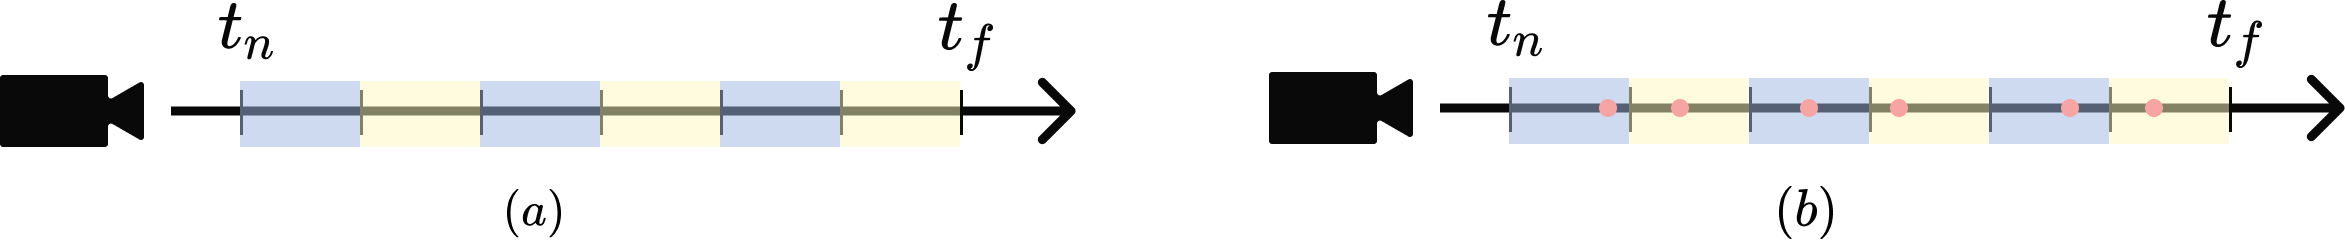
\includegraphics[width=1.0\textwidth]{figures/stratified-sampling.png}
    \caption[Stratified sampling]{a) The ray is uniformly binned from the near bound $t_n$ to the far bound $t_f$, defining the strata. b) A single random point is randomly sampled from each stratum.}
    \label{fig:stratified-sampling}
\end{figure}

% ✅ Somewhat rewritten
\subsubsection{Hierarchical sampling} \label{sec:hierarchicalsampling}
When training a NeRF, different sampling strategies can be utilized. The sampling strategy is an important choice as it is core to how the dataset for the \acrshort{mlp} is constructed. The original NeRF paper \cite{mildenhall_nerf_2020} proposed the use of a sampling approach called hierarchical sampling. This method involves training two MLPs: a \textit{coarse} \acrshort{mlp} and a \textit{fine} \acrshort{mlp}. During training, the coarse \acrshort{mlp} employs stratified sampling which involves uniform interval sampling within each bin along the ray. The coarse \acrshort{mlp} outputs a \acrfull{pdf} that highlights the samples that significantly contribute to the final predicted RGB value. This \acrshort{pdf} is then passed to the fine \acrshort{mlp} which sample points along the ray in accordance with the \acrshort{pdf}. This strategy of having a coarse network predict the important areas to sample, i.e. the regions containing volume, facilitates the fine network in generating improved predictions.

% Point from Mip-NeRF 360. Doesn't fit very well here, but it's a good point!
%The only reason why the coarse network is supervised is to guide the sampling of the fine network. This is the motivation behind improvements in e.g. Mip-NeRF 360



An overview of the NeRF pipeline can be viewed in \autoref{fig:nerf-pipeline}

\begin{figure}[h]
    \centering
    %\hspace*{-48px}
    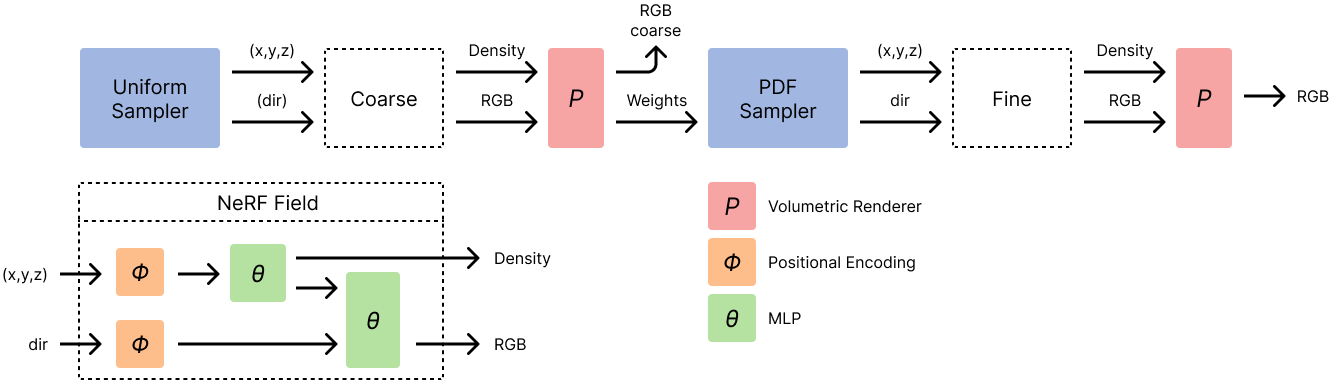
\includegraphics[width=1.0\textwidth]{figures/nerf-pipeline-overview.png}
    \caption{Overview of the NeRF pipeline}
    \label{fig:nerf-pipeline}
\end{figure}


% --------------------- Structure from motion ---------------------
\section{COLMAP (Structure from Motion)} \label{sec:colmap}
% ✅ Rewritten
\acrshort{sfm} is a technique for estimating 3D structures from sequences of 2D input images. Although some NeRF approaches have  endeavored to eliminate the necessity for pose supervision \cite{lin_barf_2021}\cite{wang_nerf--_2022}, accurate camera poses are typically a strict requirement in most NeRF methods. As a result, SfM techniques may be employed as a preprocessing mechanism for retrieving the camera poses of the input images.

% TODO: Add section about how BaRF and NeRF-- both only work on object-centric scenes.

% OLD
%Structure from motion is a technique for estimating 3D structures from sequences of 2D input images. In NeRF it can be used as a preprocessing tool for retrieving camera poses of the input images. In most NeRF methods, accurate camera poses are a strict requirement, although some papers have experimented with removing the need for pose supervision \cite{lin_barf_2021}\cite{wang_nerf--_2022}.

% ❌ Pretty happy with how this reads. Haven't changed anything
%\subsection{COLMAP} \label{sec:colmap}
COLMAP is a general-purpose SfM \cite{schonberger_structure--motion_2016} and \acrfull{mvs} \cite{schoenberger2016mvs} pipeline. The general overview of the pipeline contains the following steps:
\begin{enumerate}
    \item Feature detection and extraction
    \item Feature matching and geometric verification
    \item Structure and motion reconstruction
\end{enumerate}

During the first step, \acrfull{sift} \cite{lowe_distinctive_2004} is used to extract features in the images. This algorithm finds sparse feature points in the image and describes their appearances using numerical descriptors.

% TODO: Elaborate on the different match-options; Exhaustive Matching, Sequential Matching, Vocabulary Tree Matching. Runtimes, found in the paper, can be added to appendix.

During the second step, features are matched. Correspondences between the feature points are matched across different images, leveraging feature matching and geometric verification. There are different options for matching algorithms. \textit{Exhaustive matching} would match every image against every other image, leading to the best reconstruction results. The time complexity is not an issue if the number of images is relatively low (several hundreds). Another option is \textit{sequential matching} which is useful if the captured images are in sequential order, e.g. if they're sampled from a video.

During the third step, structure and motion is reconstructed. First, COLMAP will generate a sparse reconstruction of the scene, extracting the camera poses (camera extrinsics). The sparse output serves as input to the \acrfull{mvs} to recover a dense representation of the scene. The dense representation estimates the dense surfaces. In NeRF-applications, COLMAP is primarily used as a preprocessing step for retrieving the camera poses of input images. Because of this, the pipeline is usually ceased after the sparse reconstruction.

\begin{table}[h] 
\centering
\begin{tabular}{lcc}
\hline
Matching algorithm & \multicolumn{1}{l}{Time complexity} & \multicolumn{1}{l}{Space complexity} \\ \hline
Exhaustive         & $\mathcal{O}(n^2)$       & $\mathcal{O}(n^2)$  \\
Sequential         & $\mathcal{O}(n k)$ & $\mathcal{O}(n k)$        \\
Vocabulary Tree    & $\mathcal{O}(n^2)$       & $\mathcal{O}(n k)$  \\ \hline
\end{tabular}
\caption[Time and memory complexities of COLMAP matching algorithms.]{An overview of the time and memory complexities of a selection of COLMAP matching algorithms. For sequential matching $k$ is the number of adjacent images each image $n$ is matched against. For Vocabulary tree-based matching, $k$ is the number of top-retrieved images that each image $n$ is matched against.}
\label{tab:colmap-feature-complexity}
\end{table}

\begin{comment}
Exhaustive matching:
time complexity: O(n^2), where n is the number of images
memory complexity: O(n) for storing all images, O(n^2) for storing the results of the matching process

Sequential matching:
time complexity: O(n * k), where n is the number of images and k is the number of adjacent images each image is matched against
memory complexity: O(n * k)

Vocabulary tree-based matching:
time complexity: O(n^2), assuming that the size of the vocabulary tree is constant and not a function of the number n of images
memory complexity: O(n * k), where k is the number of top-retrieved images that each image is matched against
There is definitively literature on the topic of the time and memory complexity of vocabulary tree-based matching and image retrieval
\end{comment}

\section{Nerfstudio} \label{sec:nerfstudio}
%Since publication of the original NeRF paper, a multitude of different methods regarding NeRF has been published. Some of the papers are published with corresponding source code and some not. However, it's no easy task to compare the different methods on self-captured data. Nerfstudio is an open-source framework/API that 

Since the publication of the original NeRF paper \cite{mildenhall_nerf_2020}, a multitude of different methods regarding NeRF has been published. With the magnitude of published methods, some with corresponding source code and some not, it's not trivial to compare them on self-captured data. Nerfstudio \cite{nerfstudio} is an open-source framework/API that streamlines the process, training, evaluation, and rendering of NeRFs. The components that make up NeRFs are modularized in a way that allows interpretable implementation of different NeRF methods. In addition, Nerfstudio ships with implemented versions of some of the most important published methods to date for real-world captures. The core concepts within Nerfstudio are presented in \autoref{fig:nerfstudio-pipeline-components}. 

\begin{figure}[!h]
    \centering
    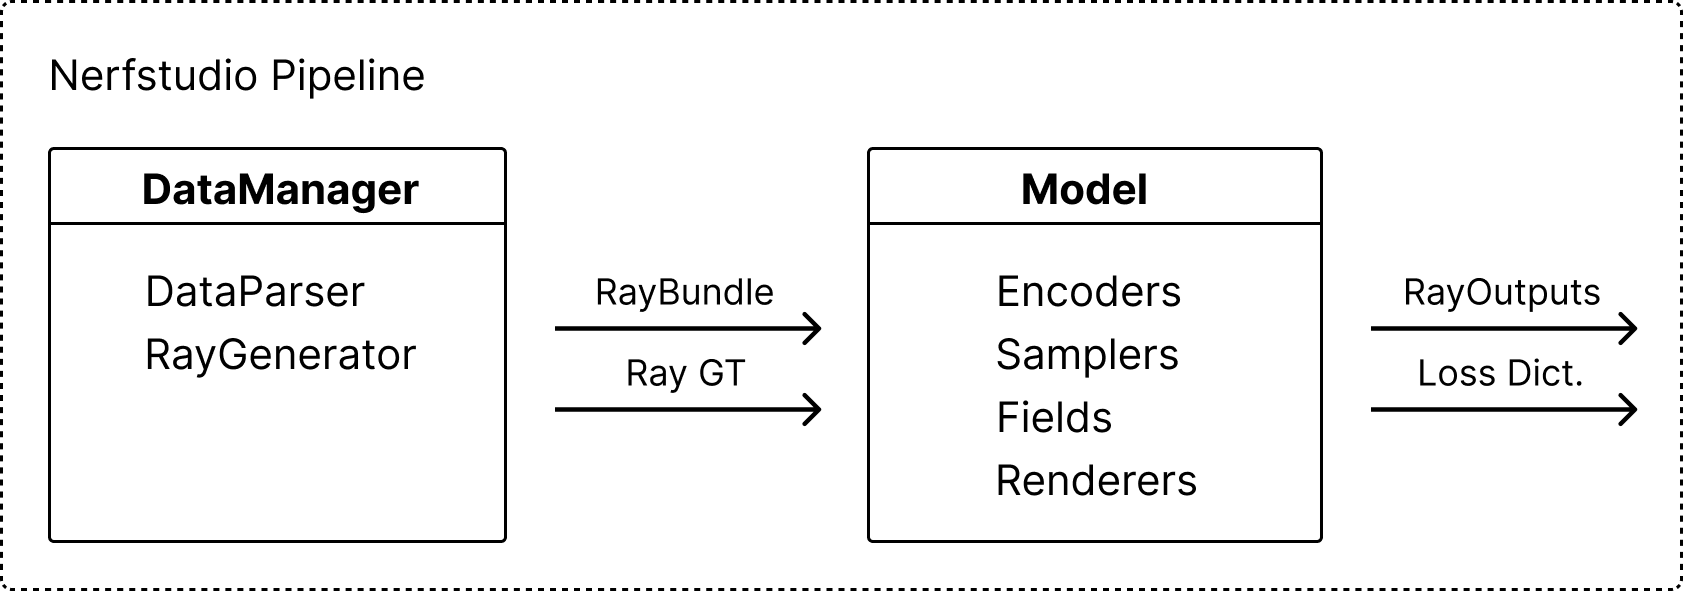
\includegraphics[width=1.0\textwidth]{figures/nerfstudio-pipeline-components.png}
    \caption[The components of the Nerfstudio pipeline.]{The components of the Nerfstudio pipeline. \texttt{DataManager}s process input images into bundles of rays (\texttt{RayBundles}) that are rendered by the \texttt{Model} to produce a set of NeRF outputs (\texttt{RayOutputs}). A dictionary of losses supervises the pipeline. Figure and caption adapted from Figure 2 in \textit{Nerfstudio: A Modular Framework for Neural Radiance Field Development} \cite{tancik_nerfstudio_2023}.}
    \label{fig:nerfstudio-pipeline-components}
\end{figure}

%\textbf{\texttt{DataManagers} and \texttt{DataParsers}}:



\section{CARLA} \label{sec:carla}
CARLA \cite{Dosovitskiy17} is an open-source simulator for \acrshort{ad} research which enables the capture of synthetic data in a controllable and programmable environment. Its highly customizable simulation environment allows for the creation and testing of a wide range of driving scenarios and conditions. CARLA includes a variety of sensors, such as cameras, \acrfull{lidar}, and \acrfull{gps}/\acrfull{gnss}, which can be used to collect both visual and non-visual data. We can interact with the CARLA simulator via a Python API, which allows for the control of vehicle position, orientation, and most other behaviors within the simulation. This flexibility enables the generation of diverse and realistic data, making CARLA, among many other things, a powerful tool for the development and testing of data capture pipelines. Data captured from CARLA can be seen in \autoref{fig:carla-3-camera-setup}.

\begin{figure}[ht]
    \centering
    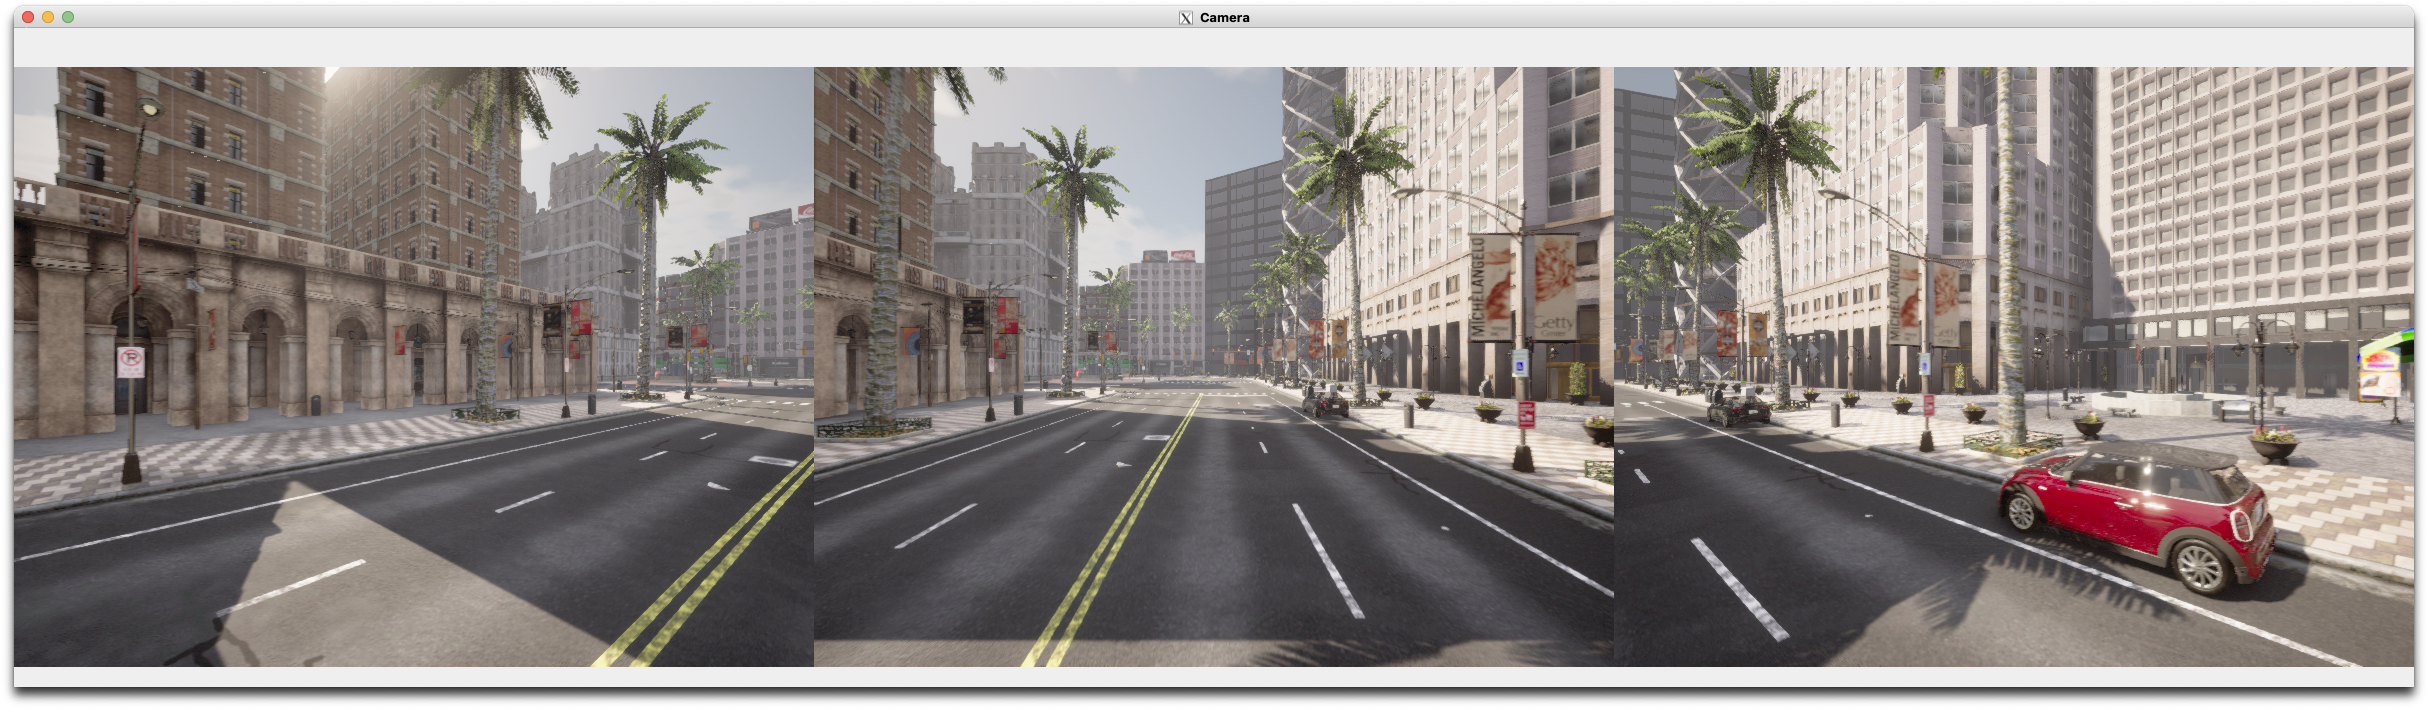
\includegraphics[width=1.0\textwidth]{figures/carla-3-camera-setup.png}
    \caption[Screenshot from the CARLA simulator.]{A screenshot from a simulation in the CARLA environment where a car has been equipped with three cameras with different rotations. The output from the mounted cameras have been horizontally stacked and rendered with OpenCV\cite{opencv_library}.}
    \label{fig:carla-3-camera-setup}
\end{figure}



% --------------------- Evaluating NeRFs ---------------------
% ✅ Rewritten
\section{Evaluating NeRFs} \label{sec:evaluating-nerfs} 
Evaluating the quality of NeRFs is a difficult task due to the visual nature of the modality. Once a NeRF is trained, it is typically employed to render an image, making image similarity metrics the most critical measure for evaluating NeRF quality. The evaluation of image similarity has been a persistent challenge in computer graphics, but the following metrics are commonly used throughout most papers comparing NeRFs.

% OLD
% Evaluating the quality of NeRFs is inherently hard since it's a visual modality. After a NeRF is trained it will eventually be used to render an image. Image similarity metrics are consequently the most important metric to evaluate the quality of a NeRF. The assessment of image similarity has been a long-standing challenge in computer graphics, but the following metrics are commonly used throughout most papers comparing NeRFs.

% ✅ Not much done, already well-written subsection.
\subsection[PSNR]{\acrfull{psnr}} \label{sec:psnr}
\acrshort{psnr} is a common measure for quantifying reconstruction quality for images and videos. It builds upon \acrfull{mse} which measures the absolute difference between each pixel in two images $I_1$ and $I_2$.

\begin{align} 
    \text{PSNR} &= 20 \cdot \log_{10}\left(\dfrac{MAX_I}{\sqrt{\text{MSE}}}\right) \label{eq:psnr}, \ \text{where} \\ 
    %\\ &= 20 \cdot log_{10} (MAX_I) - 10 \cdot log_{10}(MSE)
    \text{MSE} &= \dfrac{1}{m n} \sum_{i = 0}^{m-1} \sum_{j = 0}^{n-1} \left[I_1(i,j) - I_2(i, j) \right]^2, \ \text{and} \label{eq:mse}
\end{align}

and $MAX_I$ represents the dynamic range of an image, i.e. the largest range of pixel values that the picture may contain. This is 255 when pixels are represented with 8 bits per sample. In more general terms, $MAX_I$ is $2^B-1$ when samples are recorded with $B$ bits per sample. Due to the high dynamic range of many signals, \acrshort{psnr} is typically expressed as a logarithmic number using the \acrfull{db} scale.


% ✅ Rewritten
\subsection[SSIM]{\acrfull{ssim}}
While \acrshort{mse} and \acrshort{psnr} are effective measures of reconstruction error, they do not evaluate an image in the same manner as humans. Rather than comparing pixel values in order to conclude if two images are similar, humans assess images holistically. \acrshort{ssim} attempts to replicate this approach by comparing an image's luminance $l$, contrast $c$, and structure $s$ between two windows $\pmb{x}$ and $\pmb{y}$ of a common size $N \times N$.

% OLD
%Although MSE and PSNR are good measures of the reconstruction error, they don't examine an image the same way humans do. We don't compare pixel-value to pixel-value in order to conclude if two images are similar, we look at it in a more holistic way. SSIM tries to capture this by instead comparing luminance $l$, contrast $c$ and structure $s$ between two windows $x$ and $y$ of common size $N \times N$.

\begin{align} \label{eq:ssim}
    \text{SSIM}(x, y) &= l(x,y)^\alpha \cdot c(x,y)^\beta \cdot s(x,y)^\gamma \qquad \text{with } \alpha, \beta, \gamma = 1 \\
    &= \dfrac{(2\mu_x \mu_y + c_1)(2\sigma_{xy} + c_2)}{(\mu_x^2 + \mu_y^2 + c_1)(\sigma_x^2 + \sigma_y^2 + c_2)}
\end{align}

\begin{comment}
\begin{itemize}
    \item $\mu$ represents the pixel sample mean for both $x$ and $y$,
    \item $\sigma^2$ represents the variance for both $x$ and $y$,
    \item $\sigma_{xy}$ represents the covariance of x and y,
    \item $c_1 = (k_1L)^2$, $c_2 = (k_2L)^2$ are variables to stabilize the division with weak denominator,
    \item $L$ represents the dynamic range of the pixel-values,
    \item $k_1 = 0.01$, $k_2 = 0.03$ by default   
\end{itemize}
\end{comment}

\acrshort{ssim} is bounded by $-1 \leq \text{SSIM} \leq 1$ where $1$ implies perfect correlation, $0$ implies no similarity, and $-1$ implies perfect anti-correlation.


% ✅ Rewritten
\subsection[LPIPS]{\acrfull{lpips}}
\acrshort{lpips} \cite{zhang_unreasonable_2018} is a perceptual similarity metric based on deep network activations. Unlike \acrshort{mse}, \acrshort{psnr} and \acrshort{ssim} which uses relatively shallow functions in order to determine similarity across images, \acrshort{lpips} leverages deep neural networks to obtain a metric that perceives similarity in a way that is similar to humans. 

The dataset used to train \acrshort{lpips} includes two types of perceptual judgments; \acrfull{2afc} and \acrfull{jnd}. In \acrshort{2afc}, people were asked to select which of two distorted images was “closer” to the reference, while in \acrshort{jnd}, people were presented with two image patches, one reference and one distorted, and asked if they were the same. Some samples from the dataset is depicted in \autoref{fig:lpips}. By training on this dataset, \acrshort{lpips} is able to capture higher-level features of images that are more relevant to human perception, such as object shapes and textures. This makes it a more effective similarity metric than traditional metrics like \acrshort{mse}, \acrshort{psnr}, and \acrshort{ssim}. Image patches with a low \acrshort{lpips} score are perceptually similar.

\begin{figure}[ht]
    \centering
    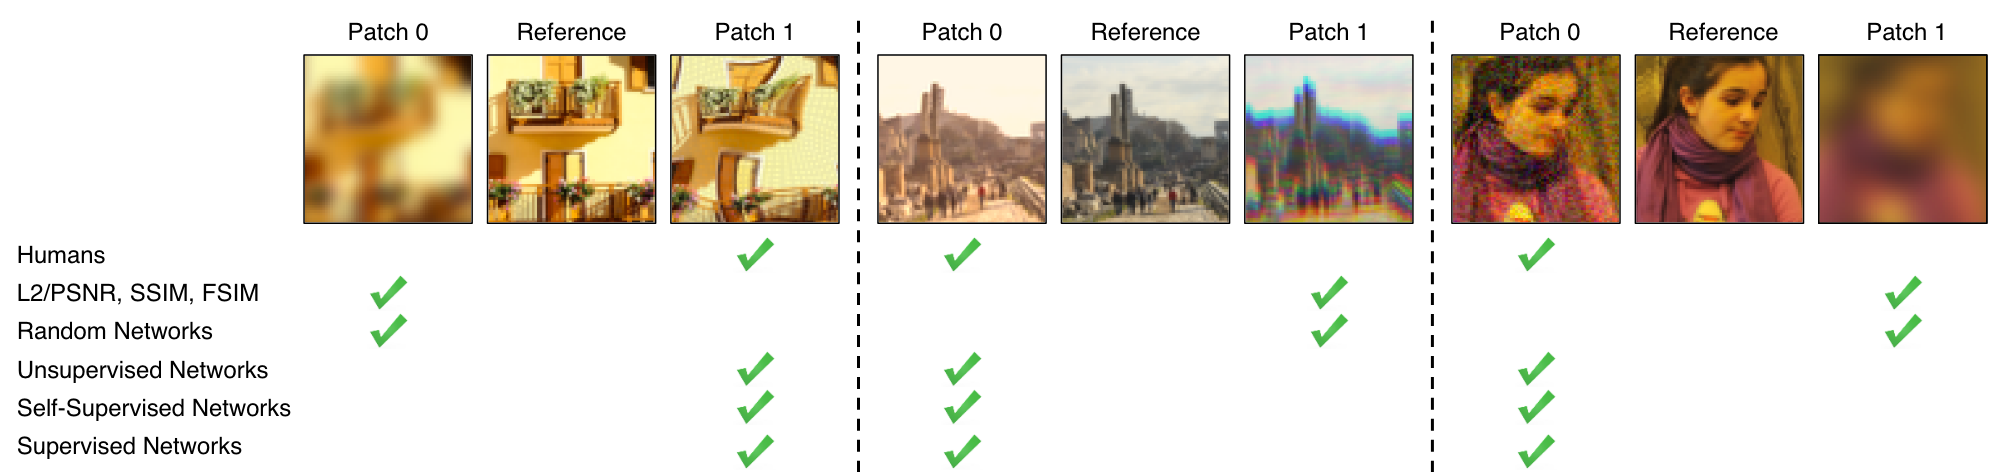
\includegraphics[width=1.0\textwidth]{figures/lpips.png}
    \caption[LPIPS - Learned Perceptual Image Patch Similarity]{\acrshort{lpips} is trained to perceive image similarity the same way humans do. The dataset used to train the similarity metric contains two types of perceptual judgements, \acrshort{2afc} and \acrshort{jnd}. With \acrshort{2afc} people were asked to select which of the distorted images was "closer" to the reference. With \acrshort{jnd} people were presented with 2 image patches, one reference and one distorted, and asked if they were the same. Figure 1 from \acrshort{lpips} \cite{zhang_unreasonable_2018}.}
    \label{fig:lpips}
\end{figure}



%The metric determines how similar two image patches' activations are, for a given network. It's been demonstrated that this metric closely matches human perception. Image patches with a low LPIPS score are perceptually similar.


\section{Related Work}
% --------------------- Other models that Nerfacto builds on ---------------------
Since the publication of the original NeRF paper, there has been a surge of related papers proposing new methods, techniques, and applications. This section covers some of the significant NeRF methods, including more specific work on the application of NeRF on vehicle-captured data.

% --------------------- mip-NeRF ---------------------
\subsection[Mip-NeRF]{Mip-NeRF: A Multiscale Representation for Anti-Aliasing Neural Radiance Fields} \label{sec:mipnerf}
NeRF demonstrates impressive performance when the training and evaluation images are captured at similar distances from the scene, without the need to account for scale or aliasing effects. When you add more cameras, pulled away from the scene, NeRF starts to deteriorate because it's a single-scale model now trying to solve a multi-scale problem. As a consequence, renderings from the NeRF exhibit aliasing artifacts in distant views and excessive blur in close-up views.

A solution to this problem would be to adopt a technique that is used in offline ray tracing, \textit{supersampling}. With supersampling, we would march multiple rays through the same pixel's footprint. This technique doesn't resolve the issue of aliasing effects, but it does result in improved visual quality of the rendered image. However, doing so would be very computationally expensive and it would further increase the lengthy training times of NeRF, which already relies on querying an underlying \acrshort{mlp} hundreds of times for a single ray.

Another sampling strategy apart from casting rays through each pixels' footprint would be to cast a cone, as seen in \autoref{fig:mip-nerf-frustums}. The cone's radius is determined by the size of the pixel's footprint on the image plane, thereby enabling the cone to model the whole volume of space visible by the pixel. When the pixel's cone is rendered, all the content within that visible volume will be averaged out, instead of rendering out whatever intersects with the infinitely narrow ray cast by NeRF. The cone is divided into conical \textit{frustums}. The frustums are approximated with a multivariate Gaussian since they're easier to manipulate and have a closed-form solution.

Instead of positionally encoding a single point along the ray, we compute the expected positional encoding with respect to the 
constructed Gaussian. With this encoding, Mip-NeRF is able to reason about the scale of its input by analyzing the scale of the encodings. This allows the model to understand the difference between small and large volumes. This encoding scheme is called \acrfull{ipe}, and has a simple closed-form solution that can be computed quickly.

\begin{figure}[ht]
    \centering
    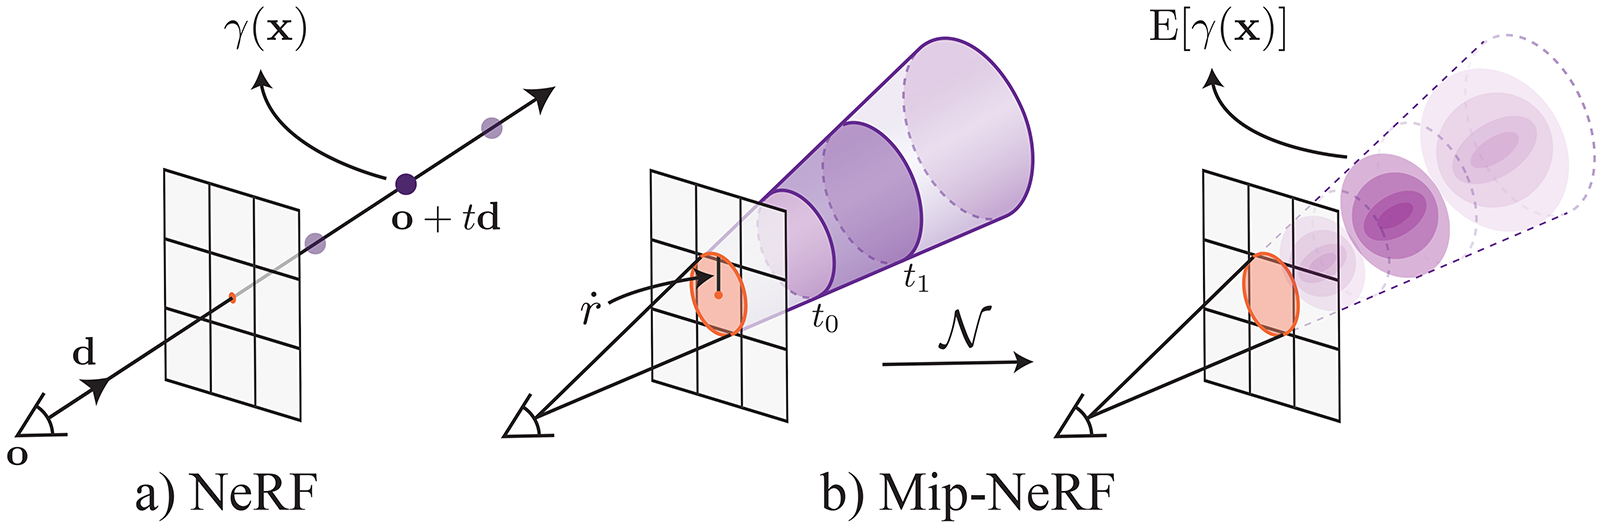
\includegraphics[width=1.0\textwidth]{figures/mip-nerf-frustums.png}
    \caption[Illustration of positional encoding]{A comparison of sampling strategies. NeRF (a) samples points along rays traced through each pixel before positionally encoding the points. Mip-NeRF (b) cast cones through the pixels' footprint and into the volume before applying \acrfull{ipe}. Figure 1 from Mip-NeRF \cite{barron_mip-nerf_2021}.}
    \label{fig:mip-nerf-frustums}
\end{figure}

This method draws inspiration from mipmapping \cite{williams1983pyramidal}, a technique traditionally used in computer graphics pipelines to mitigate aliasing artifacts. Mipmapping involves generating a pre-filtered set of discretely downsampled signals, typically images, which accelerates rendering by shifting the responsibility of anti-aliasing to a pre-computation phase. Mip-NeRF extends NeRF to simultaneously represent the pre-filtered radiance field for a continuous space of scales, thereof "Mip-NeRF".

\autoref{fig:mip-nerf-pipeline-overview} provides an overview of the Mip-NeRF pipeline. The primary distinction from the NeRF pipeline, as depicted in \autoref{fig:nerf-pipeline}, is the incorporation of the Mip-NeRF field, which utilizes \acrshort{ipe}.

\begin{figure}[h]
    \centering
    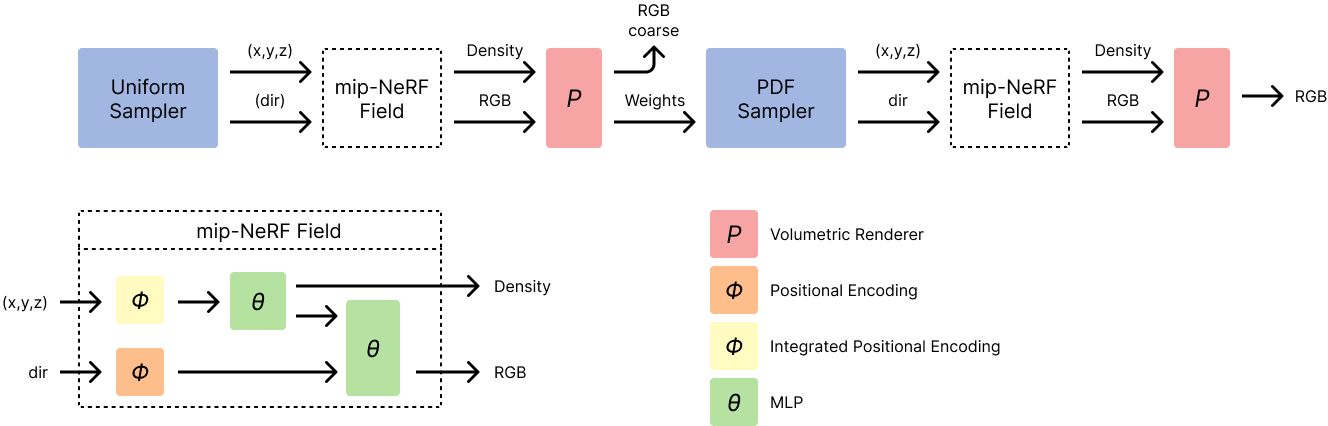
\includegraphics[width=1.0\textwidth]{figures/mip-nerf-pipeline-overview.png}
    \caption{Overview of the Mip-NeRF \cite{barronMipNeRFMultiscaleRepresentation2021} pipeline.}
    \label{fig:mip-nerf-pipeline-overview}
\end{figure}



% --------------------- mip-NeRF 360 ---------------------
\subsection[Mip-NeRF 360]{Mip-NeRF 360: Unbounded Anti-Aliased Neural Radiance Fields} \label{sec:mipnerf360}
Mip-NeRF introduces several valuable techniques for advancing the capabilities of NeRFs. However, the techniques are primarily focused on forward-facing scenes \cite{mildenhall2019llff} as opposed to unbounded scenes that are object-centric, featuring elaborate backgrounds and images captured from $360^\circ$ around the object. To extend the capabilities of Mip-NeRF to unbounded scenes, Mip-NeRF 360 \cite{barron_mip-nerf_2022} proposes three primary techniques, which are covered in this subsection.

\subsubsection{Representation}
%Problem: Unbounded scenes are large, but mip-NeF needs a bounded domain
%Solution: Apply a Kalman-like warp to mip-NeRF Gaussians to warp the mip-NeRF into non-Euclidean space.
The first challenge with extending Mip-NeRF to unbounded scenes is that such scenes are large, but Mip-NeRF requires a bounded domain. Mip-NeRF handles scenes unbounded in one direction by warping the space into \textit{projective space}, \acrfull{ndc}, but the challenge arises when the scene is unbounded in all directions. A solution is to apply a Kalman-like warp to Mip-NeRF Gaussians in order to warp the Mip-NeRF into non-Euclidean space. All the Gaussians outside a sphere of radius one will smoothly be warped into a non-euclidean space within a sphere of radius two. This non-Euclidean space is used to represent the input to the \acrshort{mlp}. 


\subsubsection{Efficiency}
%Problem: Large scenes require more network capacity, but using a large MLP is too expensive (given that you have to query it hundred of times for a single ray)
%Solution: "Distill" scene geometry from a large NeRF MLP into a small MLP while training. Train a small proposal MLP to bound the geometry predicted by a large NeRF MLP which makes training ~3 times faster
Expanding a bounded scene to an unbounded scene results in larger scenes that require a more substantial network capacity. However, using a large \acrshort{mlp} is too expensive given that it has to be queried hundreds of times for a single ray. A solution is to distill scene geometry from a large NeRF \acrshort{mlp} into a small \textit{proposal MLP} while training. The proposal \acrshort{mlp} will only output a set of weights, no colors. By feeding a set of location points through the proposal \acrshort{mlp}, the outputted weights can then be used as a \acrshort{pdf} to resample the ray, similar to how the coarse network in hierarchical sampling guides the fine network's sampling. The resampled points are then used to render a color, which as normal is supervised with photometric loss. Rather than supervising the proposal \acrshort{mlp} to accurately reconstruct the image, which is done for both the coarse and fine MLPs in Mip-NeRF, the output weights are supervised to be consistent with the output weights from the NeRF \acrshort{mlp}. This is accomplished using a loss function that encourages the outputted weight histograms to be consistent with one another. This is made possible with some strong assertions on the relation between the two distributions, which ultimately summarizes the same underlying and true distribution. This new approach to training accelerates training speeds by 300\%.

%i.e. calculate a loss that correlates the output weights from the NeRF MLP and the proposal MLP. Due to this we can have a very small proposal MLP which we query very frequently, and a larger NeRF MLP which is queried relatively few times.
%To make this work we need a loss function that encourages histograms with different bin endpoints to be consistent with one another. To achieve this we make some strong assertions on the relation between the two distributions, summarizing the same underlying, true distribution. The loss function will penalize any excess mass that violates the upper bound imposed on the proposal MLP.


\subsubsection{Ambiguity}
%Problem: 3D reconstruction becomes more ambigious as you increase the scene size. Results in more artifacts
%Solution: Utilize a novel regularizer designed specifically for mip-NeRF ray intervals. The regularizer encourages each ray's histogram to be as close to a delta function as possible. 
Reconstructing 3D content from 2D photos is inherently ambiguous since the content of unbounded scenes can be everywhere and will only be seen by a tiny number of rays. This problem becomes more pronounced as scene size increases. The original NeRF-paper partially addressed this behavior by introducing random Gaussian noise to the output $\sigma$ values, before passing them through the \acrfull{relu} \cite{agarap_deep_2019}. This stimulated densities to drift toward either zero or infinity, which slightly enhanced visual performance. However this regularization is insufficient for the more challenging task that Mip-NeRF 360 tackles. Instead, Mip-NeRF 360 introduces a novel regularizer, specifically designed for Mip-NeRF ray intervals, that encourages each ray's histogram to be as close to a delta function as possible. This regularizer reduces the occurrences of "floaters", which are semi-transparent objects that appear to be floating in space.

\begin{figure}[!h]
    \centering
    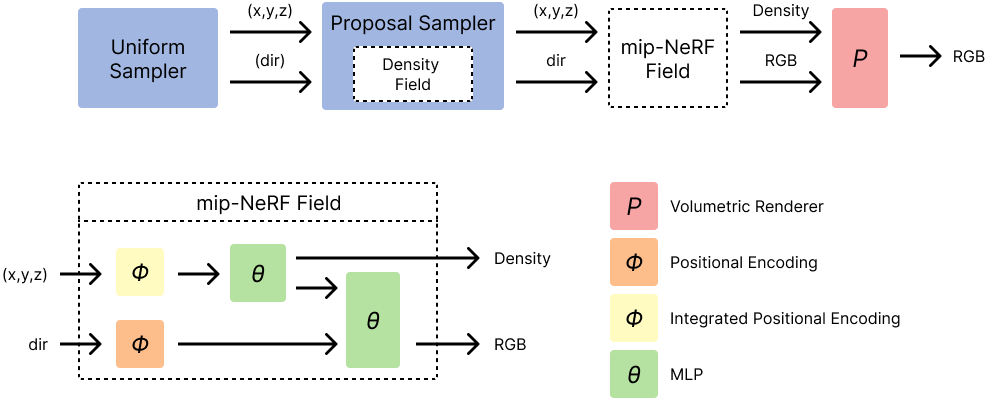
\includegraphics[width=1.0\textwidth]{figures/mip-nerf-360-pipeline-overview.png}
    \caption{Overview of the mip-NeRF 360 pipeline}
    \label{fig:mip-nerf-360-pipeline-overview}
\end{figure}

\autoref{fig:mip-nerf-360-pipeline-overview} provides an overview of the Mip-NeRF 360 pipeline, which differs in several respects from the previous Mip-NeRF pipeline depicted in \autoref{fig:mip-nerf-pipeline-overview}. Notably, the pipeline does not render a redundant RGB value, and instead features two distinct fields: a density field and a Mip-NeRF field.


\subsection[Block-NeRF]{Block-NeRF: Scalable Large Scene Neural View Synthesis} \label{sec:block-nerf}
Block-NeRF \cite{tancik_block-nerf_2022} is a paper that demonstrates a method for reconstructing large-scale scenes using NeRFs. This is achieved by splitting large areas into multiple blocks of a certain radius, with each block having a connected NeRF referred to as a Block-NeRF. The different Block-NeRFs are trained on images within their respective radius of responsibility. At inference time, only the Block-NeRFs with a radius that spans the requested location are kept. These have all been trained on image data from the requested location and can render an output. Some of the remaining Block-NeRFs might still lack a direct line of sight to the requested location, which results in low "visibility", which will be discussed further in \autoref{sec:visibility-prediction}. These Block-NeRFs are also filtered out, resulting in a pool of Block-NeRFs with good visibility. The remaining Block-NeRFs render the given location, and their outputs are merged to render the final image output.

Block-NeRF leverages multiple techniques in order to enable the reconstruction of large scenes. These include \textit{appearance embeddings}, \textit{learned pose refinement} and \textit{visibility prediction}.

\subsubsection{Appearance embeddings} \label{sec:appearance-embeddings}
Per-image appearance conditioning is a technique that was first proposed for NeRFs in NeRF\nobreakdash-W \cite{martin-brualla_nerf_2021} and has since been employed in multiple other methods. The appearance embeddings help reduce artifacts in the scene, especially "ghosting" artifacts which present themselves as fog in the final render. The appearance embedding is a vector in a low-dimensional space, unique for every input image, that is optimized jointly with the NeRF in order to allow the NeRF to process and represent 3D scenes with variable lighting, exposures, weather, and post-processing effects. To account for these variations, the final part of the \acrshort{mlp} is conditioned by passing the viewing direction concatenated with the appearance embedding.
%The appearance embedding is concatenated with the viewing direction and passed through an MLP 

\subsubsection{Learned pose refinement} \label{sec:camera-pose-refinement}
Camera pose refinement is a technique that has been proposed to alleviate the strict requirement for accurate camera poses in NeRF. This is accomplished by treating the camera poses and intrinsics as learnable parameters and jointly optimizing them with the 3D scene representation, i.e. optimizing both the photometric loss and the corresponding camera poses. It was proposed for forward-facing scenes in \textit{NeRF\nobreakdash-\nobreakdash-} \cite{wang_nerf--_2022} and later built upon in \textit{BaRF} \cite{lin_barf_2021} to support the use on object-centric scenes. Block-NeRF leverages this technique on a per-driving-segment basis. Although it is a technique optimized for forward-facing and object-centric scenes, Block-NeRF demonstrates the technique's efficacy in reducing cloudy artifacts and increasing the sharpness and overall quality of the resulting 3D representation.


\subsubsection{Visibility prediction} \label{sec:visibility-prediction}
Visibility prediction is performed to predict whether a given point is within the line of sight of a specific Block-NeRF. The prediction is made by a secondary \acrshort{mlp} $F_v$ that is trained to learn an approximation of the visibility of a sampled point. Given a location and a viewing direction, $F_v$ outputs an approximation of that location's transmittance ($T$ in \autoref{eq:volume-rendering}). The transmittance of a location will be close to 1 if it's visible, i.e. located in free space or on the surface of the first intersected object. Objects inside or behind the first intersected object will have a transmittance close to 0. If the point is visible from multiple viewing directions, the resulting transmittance will be the average of these observations. $F_v$ is supervised by the Block-NeRF's main \acrshort{mlp} $F_\sigma$.



% --------------------- Instant-ngp ---------------------
\subsection[Instant-ngp]{Instant-ngp: Instant Neural Graphics Primitives with a Multiresolution Hash Encoding} \label{sec:instant-ngp}
Instant-ngp \cite{muller_instant_2022} is a paper that introduces a method for accelerating the training- and inference of NeRFs. Previous NeRF methods have required hours or even days of training to learn a scene, but the team at Nvidia was able to significantly reduce both the training- and inference time while maintaining the same level of quality. This achievement represented a significant advancement in the field of NeRFs, and has greatly improved the efficiency and effectiveness of NeRF-based applications.

\begin{figure}[H]
    \centering
    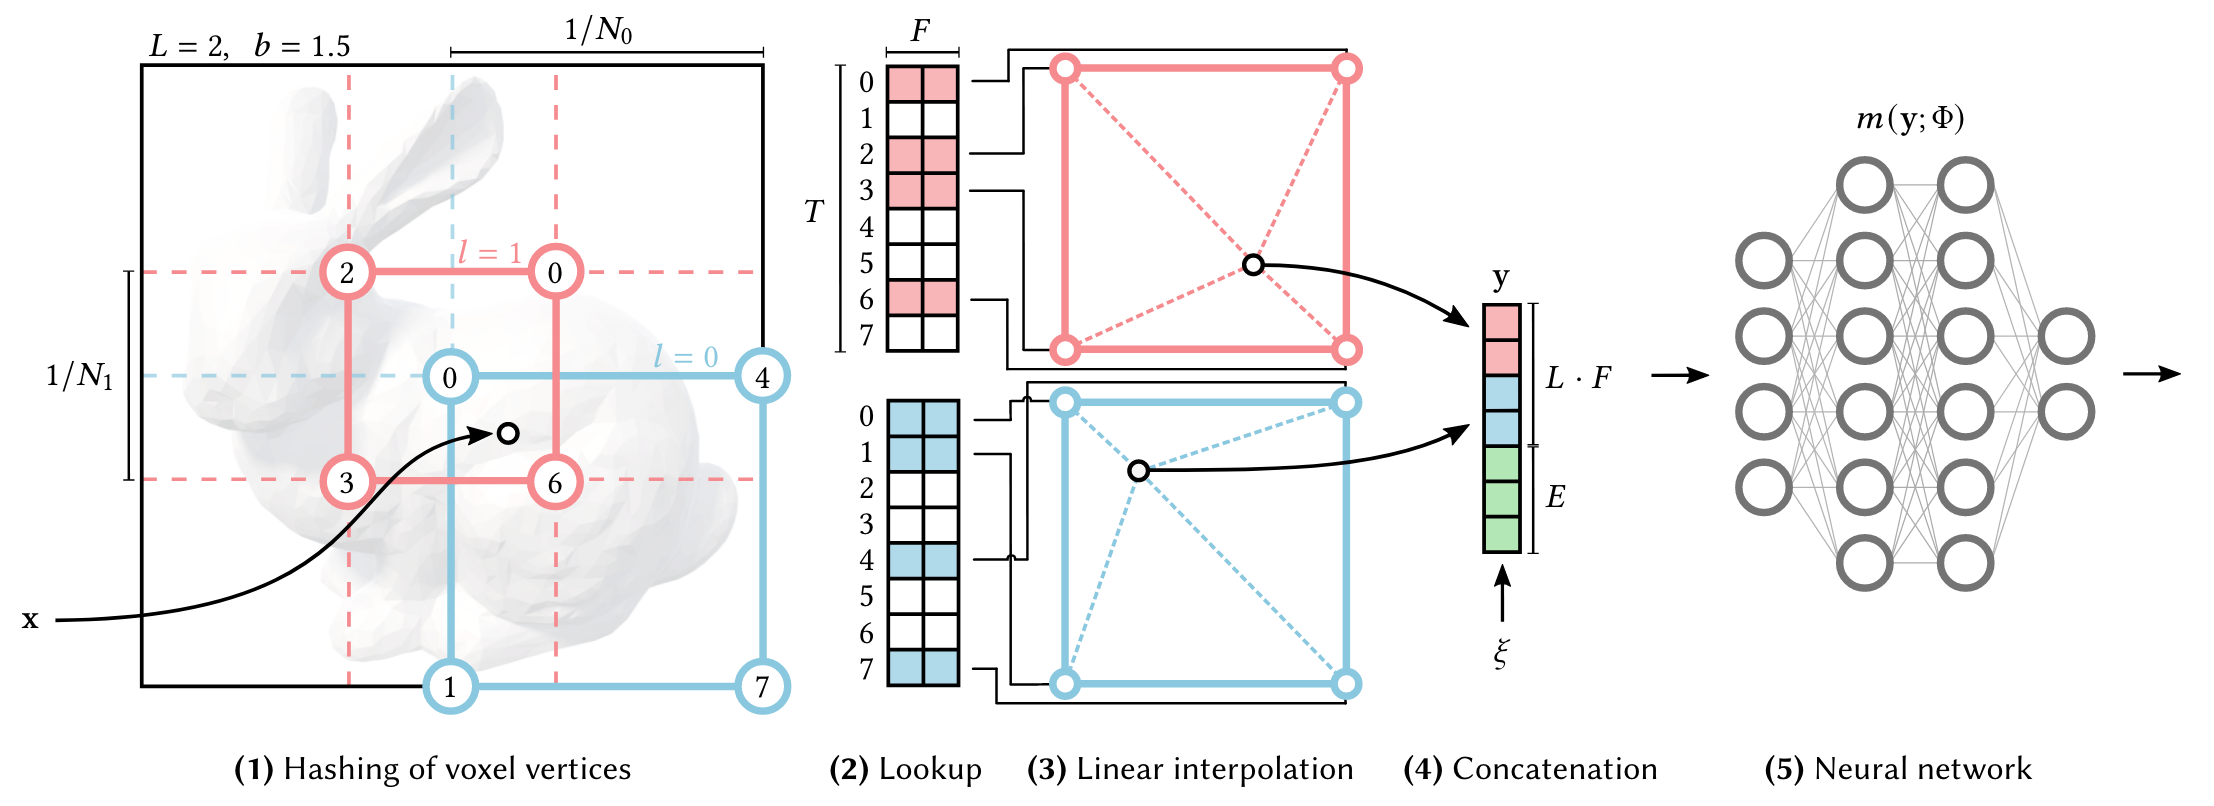
\includegraphics[width=1.0\textwidth]{figures/instant-ngp-hash-encoding.png}
    \caption[Illustration of multiresolution hash encoding]{Illustration of the multiresolution hash encoding in 2D. Figure 3 from Instant-ngp \cite{muller_instant_2022}.}
    \label{fig:instant-ngp-hash-encoding}
\end{figure}

The main technique proposed by Instant-NeRF is a new parametric encoding for the scene's spatial data, coined \textit{Multi-resolution hash encoding}. In the original NeRF paper, the location \textbf{x} is represented by a positional encoding as described in \autoref{sec:positionalencoding}. With the multiresolution hash encoding, the location \textbf{x} is represented in a hash table by a linear interpolation of its closest vertices at multiple resolutions. This parametric encoding has several advantages in terms of computational effectiveness, resulting in several magnitudes of increased training and inference speed. Although a larger memory cost is imposed by allocating several hash tables, the number of required parameter-updates per backpropagation is significantly reduced. An overview of the multiresolution hash encoding can be seen in \autoref{fig:instant-ngp-hash-encoding}.

%The only difference is essentially how spatial data is represented, i.e. parametric encoding. Instant-NGP encodes spatial data at multiple resolutions using hash tables, thereof the name multiresolution hash tables. During backpropagation, the MLP's weights and the feature vectors in the hash tables are both updated.
%In a fully connected MLP, every weight and bias must be updated on back-propagation. With parametric encodings, only a very small number of feature vectors must be updated. Also, by reducing the size of the MLP, such parametric models can be trained to convergence much faster without sacrificing approximation quality. You trade a larger memory footprint by allocating hash tables, but in return you have to update a far lower number of trainable parameters per back-propagation, leading to an increased training and inference speed.

\subsection{Nerfacto} \label{sec:nerfacto}
Nerfstudio, discussed in \autoref{sec:nerfstudio}, also provides its own method dubbed Nerfacto \cite{tancik_nerfstudio_2023}. Nerfacto leverages techniques from several other published methods that have proved to work well for real data capture. The combination of techniques, partially depicted in \autoref{fig:nerfacto-pipeline-overview}, results in a method that strikes a great balance between quality and speed. 
The primary techniques implemented in Nerfacto have already been discussed. However, they will be briefly listed and summarized in this section:

\begin{figure}[!h]
    \centering
    %\hspace*{-48px}
    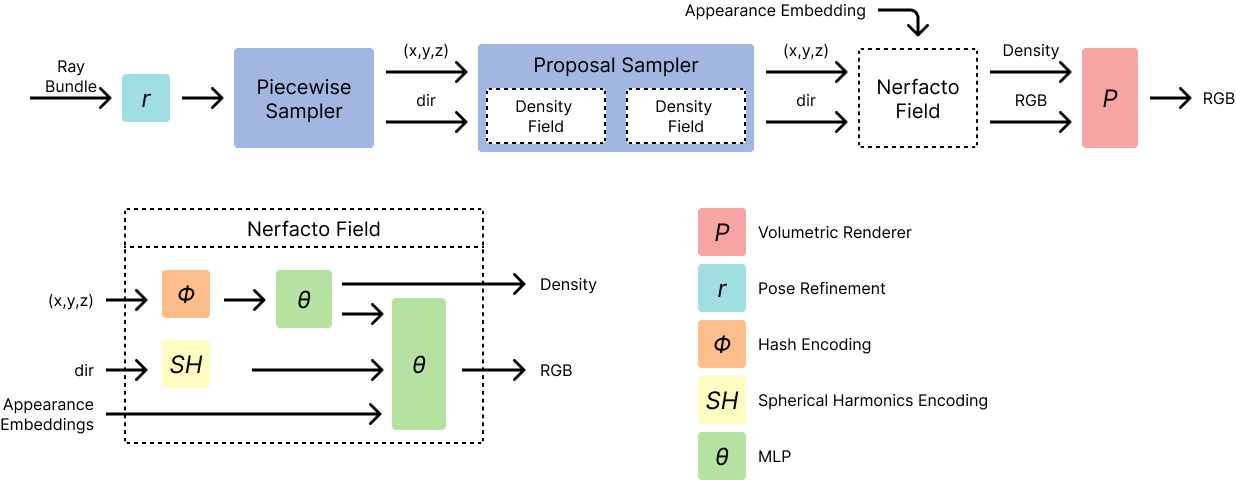
\includegraphics[width=1.0\textwidth]{figures/nerfacto-pipeline-overview.png}
    \caption{Overview of the Nerfacto pipeline}
    \label{fig:nerfacto-pipeline-overview}
\end{figure}

\textbf{Camera pose refinement}, as described in \autoref{sec:camera-pose-refinement} is a technique proposed to reduce the impact of imperfect camera poses. It's an effective measure to reduce cloudy artifacts and increase the sharpness and overall quality of the resulting 3D representation.

\textbf{Per image appearance conditioning}, as described in \autoref{sec:appearance-embeddings}, is a technique that allows the NeRF to process and represent 3D scenes with variable lighting, exposures, weather, and post-processing effects. In Nerfacto, the appearance embedding is a vector of size 32, which is concatenated with the viewing direction before it's passed through the \acrshort{mlp}.

\textbf{Hash encodings}, as described in \autoref{sec:instant-ngp}, is an effective encoding scheme used to severely decrease training- and inference time. In Nerfacto, 16 hash tables with $2^{19}$ rows, each storing a feature vector of size 2, are allocated. The subsequent \acrshort{mlp} has a very low capacity, with only one hidden layer containing 64 neurons.

\textbf{Proposal sampling}, as described in \autoref{sec:mipnerf360}, is a sampling technique used to increase the sampling density of areas that contribute most to the final render. Nerfacto extends the proposal sampler used in Mip-NeRF 360 \cite{barron_mip-nerf_2022} by utilizing two density functions implemented as small fused-\acrshort{mlp} with hash encodings \cite{muller_instant_2022}. This provides accurate and fast density estimations.

\textbf{Scene contraction}, as described in \autoref{sec:mipnerf360}, is a technique proposed in Mip-NeRF 360 \cite{barron_mip-nerf_2022} to extend Mip-NeRF to support unbounded scenes.




\subsection[Wayve - NeRFs for Autonomous Driving]{Wayve - Building City-Scale Neural Radiance Fields for Autonomous Driving} \label{sec:wayve}
Wayve, a London-based company, is a leading innovator in autonomous vehicle technology. At Nvidia GTC, they presented a talk on how they leverage NeRFs to extend their pipeline used to train autonomous vehicles. Their initial need was a simulator that was indistinguishable from reality, but building such a simulator is very time-consuming, challenging, and expensive. Their solution was to use NeRFs to automatically "build the simulator with data."

The pipeline, partially depicted in \autoref{fig:wayve-pipeline}, begins by creating a large corpus of data, captured by a specialized Wayve-vehicle fitted with high-quality cameras. The corpus is then split into data segments spanning roughly 100 meters and containing a small overlap between the previous and successive segments. In order to mask out transient objects and separate foreground and background, a segmentation model is applied to each segment. After this, each segment utilizes COLMAP to approximate the images' corresponding camera poses. Once the camera poses are acquired, each of the NeRFs are trained in parallel with an undisclosed method. Using the capture trajectory, a camera path is created and rendered by swapping NeRFs on-demand when the current camera within the path is close to another NeRF's boundary. 

\begin{figure}[!h]
    \centering
    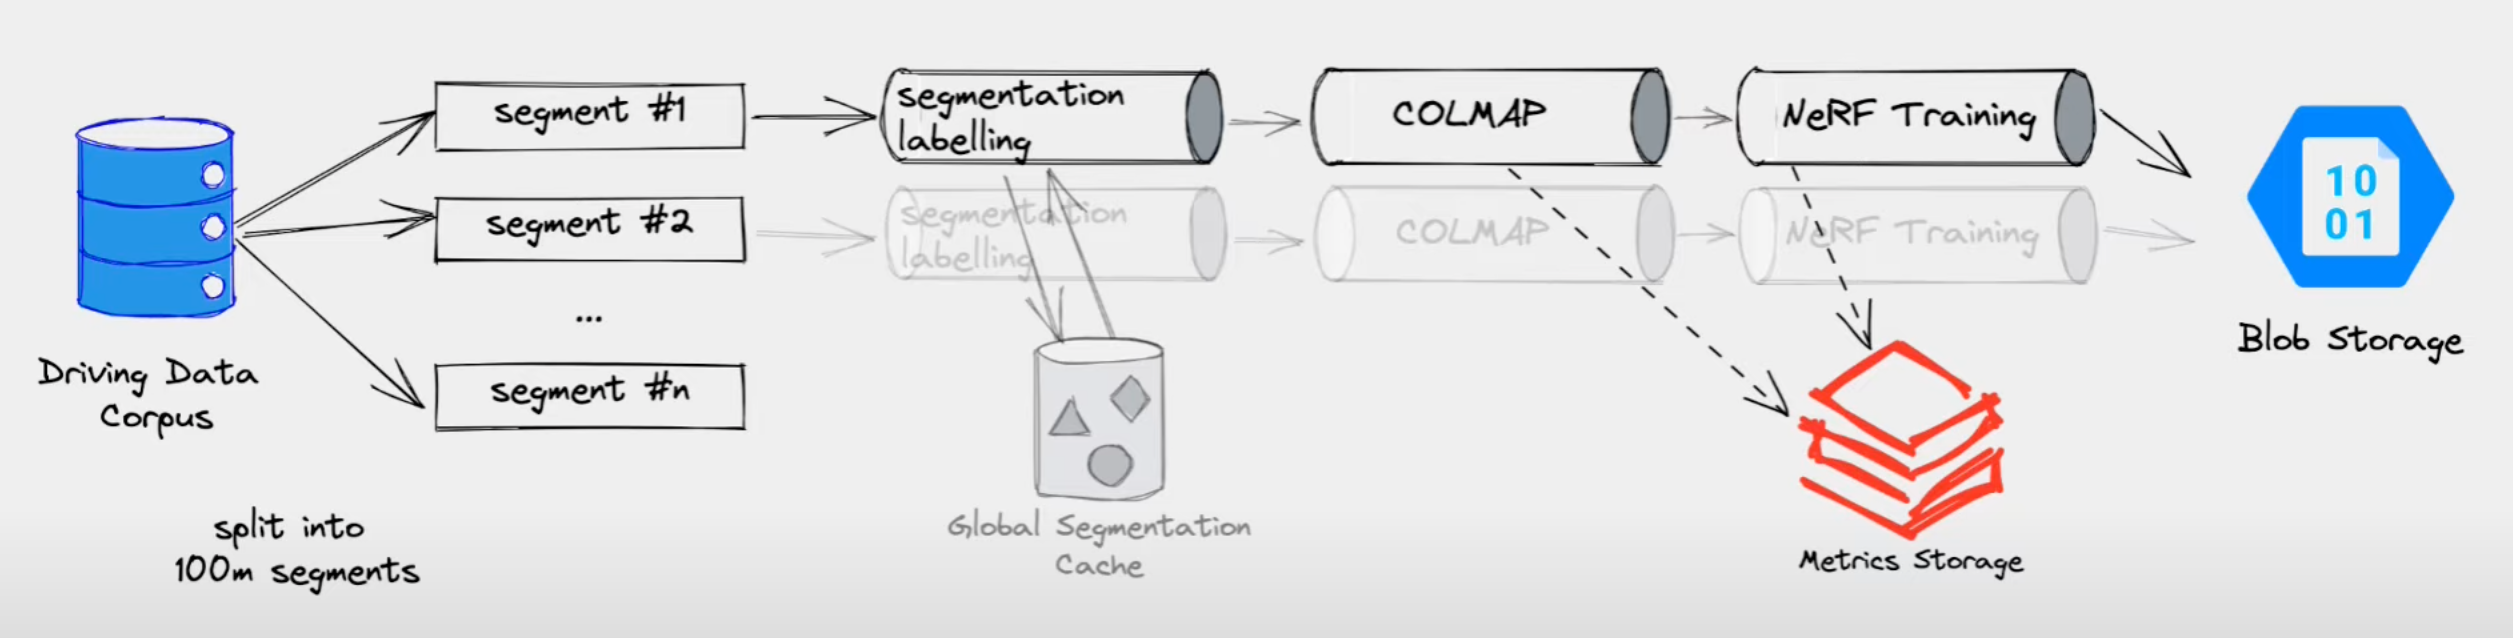
\includegraphics[width=1.0\textwidth]{figures/wayve-pipeline.png}
    \caption{An overview of Wayve's pipeline for large-scale NeRF. Image taken from Wayve's talk at Nvidia GTC \cite{sokolski2023building}.}
    \label{fig:wayve-pipeline}
\end{figure}

Wayve's pipeline is simpler and more straightforward than that of Block-NeRF because their goal is to stitch together scenes that were recorded one after the other, rather than creating a scene that can be traversed in all directions. This difference in objective allows Wayve to sidestep many of the technicalities involved in Block-NeRF making their pipeline more streamlined.